%        File: final_paper.tex
%     Created: Mon Dec 12 04:00 PM 2011 C
% Last Change: Mon Dec 12 04:00 PM 2011 C
%

%*Total number of deleterious mutations and how many of those recovered with a compensatory mutation.

%*Plot of recovery depth vs. total depth for each mutation compensated with a sign-epistatic mutation.

%*Plot of % initial fitness loss vs. depth of recovery.

%*A case study talking about the history of a single sign-epistatic interaction including a picture of it's genealogy.

%Your paper must include these things to get an "A" in the course.

\documentclass[a4paper, 10pt]{article}
\usepackage{graphicx}
\usepackage{times}
\usepackage{fullpage}
\usepackage{setspace}
\doublespacing
\begin{document}
\title{An inquiry of the role of sign epistasis in the evolution of sexually reproducing populations}
\author{Lane Smith}
\date{December 13, 2011}
\maketitle

\section{Abstract}

In this paper, the involvement of sign epistasis in the evolution of sexually reproducing populations is investigated through the use of the digital evolution software, Avida. The analysis of the data collected from the experiments is discovery, and the results provides quantitative reasons to pursue further investigation. There is substantial evidence that sign epistasis is an important factor in the evolution of the lineage leading to the dominant genotype. Evidence supporting this claim includes the large number of sign epistatic mutations that occur throughout the lineage, the persistence of sign epistatic mutations into the final dominant genome, and the relationship between fitness gains and loses in sign epistatic events and the phylogenetic depth. This research opens up possibilities to a wide variety of follow-up work, which is discussed. 

\section{Introduction \& Motivation}

A significant amount of research has been conducted investigating sign epistasis and the role of deleterious mutations in asexual populations\cite{covert}\cite{cow}. This research has shown that deleterious mutations are critical in rapid transversal of valleys in the fitness landscape. This process involving deleterious mutations is generally described as a fitness reversal, where a deleterious mutation is compensated by a separate mutation. This reversal leads into sign epistasis when together the two mutations achieve a higher fitness than either would separately. Literature comparing sign epistasis between sexual and asexual populations suggests that sign epistasis occurs with both reproductive strategies, but that recombination leads to subtly different effects\cite{visser}. On a generational scale, recombination seems to hinder the individual chance of fitness reversal, but when considered across a large population over time, recombination does not prevent escape to higher local fitness maxima\cite{weinreich}. Furthermore, recombination has not shown to confer any particular advantage when compared to asexual reproduction.

These studies consider the fitness of the population as a whole; however, the entire population will not survive and reproduce under the limitations of natural selection. The fittest (or `dominant') genotypes will reproduce more successfully and will lead to a bias of those genes in future generations. Therefore, the frequency of sign epistasis of the entire population is not as important as the frequency of sign epistasis in the lineage of the dominant genotype. It is this fact that is the basis of our investigation. We will determine the importance of sign epistatic events based entirely on what occurs and persists in the lineage of the final dominant genotype, rather than what occurs in the population as a whole.

The greatest advantage in computational evolution research must be the ability to generate large data sets quickly with as much finely-tuned detail as one desires. In contrast with a wet-lab investigating similar concepts with single-celled organisms which takes years and does not provide complete data, we use Avida, the digital evolution software used for research in digital evolution and population genetics. Avida creates a virtual world populated by digital `organisms' with unique genetic sequences that compete for limited resources. Each `organism' can be imagined as a very simple computer that performs operations as defined by it's genetic sequence. The genetic sequence is a set of basic operations that, in the proper sequence, code for the reproduction of the `organism' and other possible tasks.  The resource, for which individuals compete, is a portion of CPU cycles available in each update of Avida. A CPU cycle will allow an organism to progress through its genetic sequence. Fitness of an organism is calculated base on the organisms ability to complete logical task operations, based on their sequence of instructions; more complex logical tasks have a higher award multiplier. Organisms with higher fitnesses are rewarded with more CPU cycles, thus allowing for more fit organisms to more quickly complete its sequence of instructions and to reproduce.

The motivation for this research is to both extend prior knowledge about the mechanics of sign epistatic mutations and to inspire further research into the exact conditions and mechanics involving sign epistatic mutations in sexually reproducing populations. This research has provided a solid backing for the importance of sign epistatic mutations in the lineage of the dominant genotype. Extensions of this research will provide more definitive experiments are made to determine the exact interactions of sign epistasis in sexual reproduction. With this knowledge, we will have filled in another piece of the puzzle as to why sexual reproduction, with it's two-fold reproduction cost and myriad of impracticalities, is the most common method of reproduction in biology. 

\section{Methods}
All data was generated using Avida. Five data sets were generated with different random number seeds and run for 100,000 updates. No modifications were made to the environment, and the bounds of the virtual world was set to the default of 100 x 100. Under these conditions, Avida produces a large output file that lists all genotypes that exist at the end of the instance and all ancestor genotypes of these genotypes. This output enables us the ability construct a complete lineage of any given genotype and to analyze the specific sequence of mutational steps throughout its evolution. 

Since Avida is most often used for research with populations that reproduce asexually, modification to the source code of Avida was necessary in order to create our desired output. In Avida, `gametes' produced by each parent are duplicates of their parents' sequences with a certain probability of single substitution mutation occurring in each gamete sequence. The gametes are then randomly bisected at the same point in each sequence, and a section of each gamete is randomly selected and joined together to produce the offspring genotype. This is the process of sexual recombination the key feature that divides sexual and asexual reproduction. The resultant offspring's sequence thereby contains an average of half of each parent's sequence. The Avida source code was modified to keep track of mutations that may be carried over in recombination and to output the point at which the sequences are bisected.

Consequentially, the ability to produce massive and complete data sets in computational biology is the source of both a great strength and a great difficulty. With large data sets, considerations of algorithm complexity and resource limitations must be taken into consideration. This is especially true of a data set produced with sexual reproduction. Unique genotypes are created each time two dissimilar genotypes sexually recombine, leading to many more entities than would asexual reproduction create in the same conditions. Thus, it was important to use the most appropriate data structures and algorithms in analyzing the data created by Avida.

The process for analyzing the data set was as follows: each line of the detail file was parsed, the details of each genotype packed into a wrapper object, and the object added to a hash-map with the ID of the genotype as key. The hash-map data structure was selected because it provides constant-time ($0(1)$) access to each object at the expense of increased memory usage. Avida provides the parents of each genotype, but not the children. Using a breadth-first search algorithm, the lineage starting from the dominant genotype to the original genotype was traced and a list of each genotype's children added to their  respective object. All genotypes not directly related to the final dominant genotype were pruned, thus helping to keep the required memory lower. 

To search for deleterious mutations, a breadth-first search algorithm is used to start at the top of the lineage (the original genotype) and to search each genotype in succession for an potentially deleterious mutation. When a deleterious mutation is suspected, this is verified by running the sequence through Avida to determine the fitness of the sequence with the mutation and with the mutation reverted. If the mutation is indeed deleterious where the sequence had a higher fitness with the mutation reverted, we investigate this mutation as a candidate for sign epistasis. 

Starting from the origin of the deleterious mutations, we search through each of the genotype's descendants in a breath-first search manner. If the deleterious mutation persists in an offspring and the offspring contains a new mutation, we investigate the effect of reverting the deleterious mutation. This investigation is performed similarly to distinguishing a deleterious mutation by comparing the values of fitness for the mutation present and reverted as output from Avida in analyze mode. Unlike the previous comparison, if the fitness of the genotype is higher with the initially deleterious mutation than with it reverted, we recognize this as a sign epistatic event. We then determine whether the sign epistatic mutations persist through the lineage and is present in the final dominant using another breath-first search method. Details of both the genotypes at which the mutation originated and recovered are output, along with details of their parents, the total phylogenetic depth at which the mutation originally occurred, the relative phylogenetic depth between the origin and the recovery, and whether the mutation is present in the final dominant genotype. 

This process of investigating deleterious mutations for possible sign epistatic events repeats for each genotype in the lineage of the final dominant genotype, and all details written to a file. A summary of the total deleterious mutations present and the number of sign epistatic events is also output. From these files, we can create graphs and perform calculations from which to gather conclusive results. All post-analysis processes and graph creation was performed using Python and the matplotlib library.

%In order to visually understand the progression of a deleterious mutation through the lineage, we constructed a case study to examine the path of a deleterious mutation from origin to fitness reversal. A sign epistatic event was singled out from the analysis output that met the following criteria: 1) the mutation persists and is present in the final dominant genotype; 2) both the deleterious mutation and its reversal impart a large change in fitness; 3) The relative phylogenetic depth is greater than 5. A case fulfilling these requirements was curated from the data sets manually, and the graph was generated processed by means of a periphery function of the analysis script.

\section{Results}

We have gathered notable evidence that sign epistatic events play an important role in the evolution of the final dominant genotype, based on their ubiquity in the ancestral lineage of the final dominant genotype. As summarized in Table \ref{sumTable}, we see that in all 3 data sets, there are large numbers of deleterious mutations that occur in the lineage. Of these deleterious mutations, we see that there are a lesser, but still significantly high, number of these deleterious mutations that are involved in sign epistatic events. Also worth of note is the number of sign epistatic mutations that persist and are present in the final dominant genotype. 

\begin{table}[h]
    \centering
\begin{tabular}{| l || c | c | c | c |}
\hline
& {\em Trial 1} & {\em Trial 2} & {\em Trial 3} & {\em Aggregate Total}\\
\hline
Total Deleterious Mutations & 44177 & 37082 & 45843 & 127102\\
Total Sign Epistatic Mutations & 520 & 360 & 503 & 1383\\
Sign Epistatic Mutations in Final Dominant & 23 & 13 & 44 & 80\\
\hline
\end{tabular}
\caption{Summary Figures from Analysis of Trials}
\label{sumTable}
\end{table}

While this is not conclusive evidence that sign epistatic events are critical in the evolution of the final dominant genotype, it does provide us with several indications that sign epistasis plays an important role in the process of its evolution. To further investigate the relationship between sign epistasis and the evolution of the final dominant, we need to consider the relationships between all aspects of sign epistasis. This will be conducted graphically, using the aggregate data from all of the 3 trials, in order to identify trends and potential topics of interest for further investigation.

Figure \ref{totalDepth} demonstrates the relationship between the total phylogenetic depth and the relative phylogenetic depth between the origin genotype of the deleterious mutation and the genotype at which the deleterious mutation underwent reversal. This graph contains all of the points from each of the 3 trials. Total phylogenetic depth is the number of generations from the original genotype used to start the simulation to any particular genotype. Relative phylogenetic depth is the number of generations between any two directly related genotypes. 

\begin{figure}[h]
    \centering
    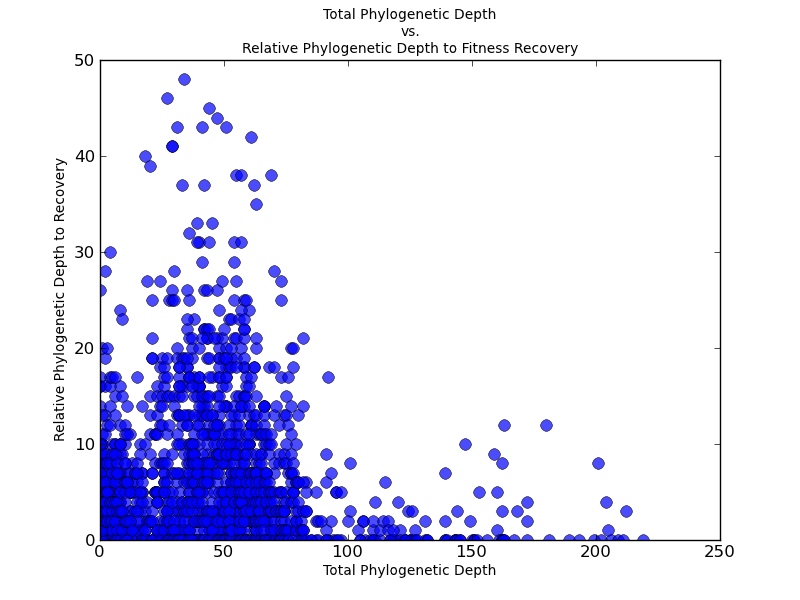
\includegraphics[scale=0.6]{totalDepth_vs_recoverDepth.png}
    \label{totalDepth}
    \caption{Comparison between the total phylogenetic depth and the relative phylogenetic depth between deleterious mutation origin and reversion}
\end{figure}

From this graph, we can see that the large majority of the sign epistatic events occur within 100 generations from the start of the trial. Furthermore, fitness reversals most often occur within 10 generations. We can see that there appears to be a negative relationship between the total phylogenetic depth and the relative phylogenetic depth to recovery; however, more data will need to be collected along with regression tests before any further results can be drawn.

Logically, we can expect that the greater loss of fitness in the genotype that originates the deleterious mutation will have an effect on the time it needs to recovery. With a greater loss in fitness relative to the fitness of the entire population, it is more likely that the genotype will be selected from the population. It follows that fitness reversals must then occur quickly if the fitness is greatly impacted. Figure \ref{fitLoss} demonstrates this trend. We can clearly see that large decreases in fitness as a percentage of the parent with the higher fitness are much more quickly reverted, and that there are very few mutations that both greatly detriment fitness and are reverted after more than 20 generations. There are some particularly interesting cases within our data that resist this trend. It might be that sexual recombination might mitigate the effect of any one deleterious mutation, allowing it to persist and later be reverted. How else could a deleterious mutation with a nearly 100\% decrease in fitness survive to be reverted more than 20 generations later? This would be an appropriate topic for further investigation.

\begin{figure}[h]
    \centering
    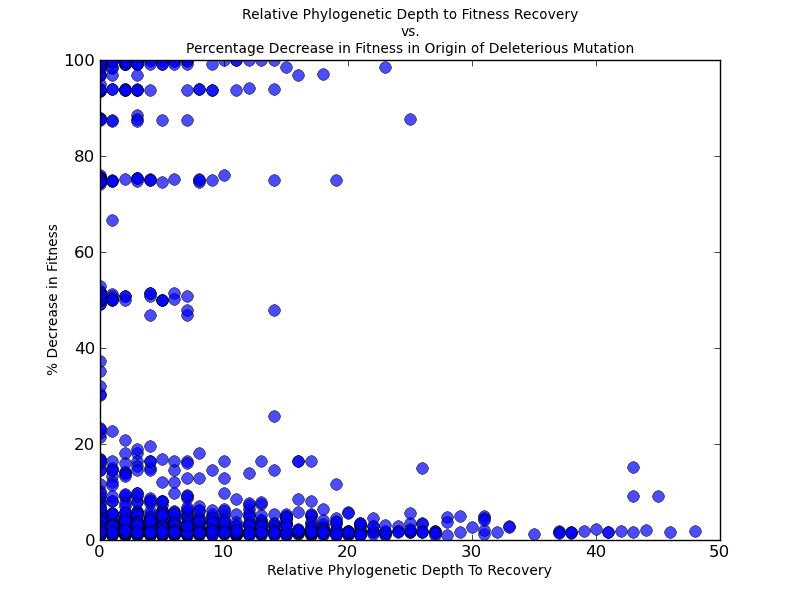
\includegraphics[scale=0.6]{initFitLoss_vs_depthRecover.png}
    \label{fitLoss}
    \caption{Comparison of the initial loss of fitness as a percent and the relative phylogenetic depth between deleterious mutation origin and reversion}
\end{figure}

For a sign epistatic event to persist for a long time, it would need to contribute a significantly beneficial effect that is unique within the population. This is precedent from the concept of fixation and the transversal of fitness valleys to higher fitness peaks. It is then worthy to investigate the relationship the percentage increase in fitness and the phylogenetic depth to the final dominant genotype. From this investigation, we produce the following figure \ref{inFD}.

\begin{figure}[h]
    \centering
    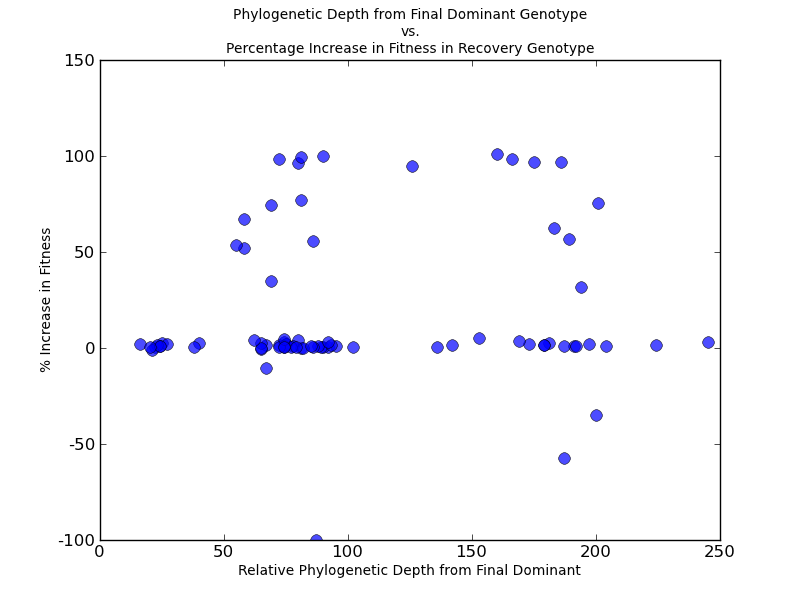
\includegraphics[scale=0.6]{fitnessInc_vs_FDDepth.png}
    \label{inFD}
    \caption{Comparison of the increase of fitness after a sign epistatic event occurs and the phylogenetic depth (distance) from the final dominant genotype}
\end{figure}

In this graph we compare the phylogenetic depth from the final dominant genotype, {\em i.e.}, values closer to 0 are closer genealogically to the final dominant genotype, to the percentage increase of fitness to in the genotype that reversed the deleterious mutation. The data points included in this graph are only those mutations that persist and are present in the final dominant genotype. The percentage increase of fitness was calculated based upon an average of the fitnesses of the two parents; a more accurate value would compare fitnesses only to the parent from which the deleterious mutation was inherited. This does not invalidate the overall trend, which shows that sign epistatic events with both dramatic and modest increases in fitness persist in the final dominant genotype.

\section{Conclusion \& Discussion}

The results provided by this research provide us with ample evidence that sign epistatic mutations are important in the evolution of the dominant lineage. We demonstrated that there is a large number of deleterious mutations that occur throughout the lineage and that a small but considerable fraction of these mutations are later involved in sign epistatic interactions. There is an inverse relationship between the total phylogenetic depth at which a deleterious mutation occurs and the relative phylogenetic depth before the fitness effect is reversed. We can confirm that there is a relationship between the loss of fitness caused by a deleterious mutation and phylogenetic depth before it is reverted. More detrimental deleterious mutations are shown to  revert more quickly than less severe mutations. Finally, the sequence of the final dominant genotype contains many nucleotides originally derived from deleterious mutations that underwent sign epistasis. The relative phylogenetic depth between the dominant genotype and reversion was compared to the fitness benefit gained from the sign epistatic event. The sequence contains many sign epistatic mutations that range widely in the benefit they gained from reversion,but we can see evidence that sign epistatic events with large gains in fitness persist for long phylogenetic depths to end in the final dominant genotype.

The most exciting aspect of this research are the opportunities that it opens up to extension. The output from the analysis script in its current form alone offers up a trove of information. For example, worthy investigations might compare the relative phylogenetic depth with the difference of origin and recovery fitness, whether the deleterious mutation or its reversion is has a lower/higher fitness than both parents, and calculating the total number of different nucleotides between the origin and the recovery genotype and plotting against the relative recovery depth. 

An inquiry that holds my personal interest is in determining how frequently sign epistasis occurs not by a new mutation, but by a recombining the deleterious mutation with part of a sequence that contains the necessary part to induce sign epistasis. While attempting to follow the lineage of a genotype that had undergone sign epistasis in a case study, I realized that the compensatory mutation in the genotype marked as the recovery genotype was, in fact, synonymous. While the inclusion of these sorts of mutations is an error in my analysis script, this was still an actual occurrence of sign epistasis. The originally deleterious mutation had indeed reversed its effect. The only way this can occur is if the contribution from the other parent made it sign epistatic.

The investigation of the role of sign epistatic events in sexually reproducing populations has only begun. This research accomplished its goal of discovering whether there was any evidence of sign epistatic mutations being of importance in the dominant lineage. We can say that, while there is significant work still yet to be accomplished before being conclusive, this research gives reasonable support to a hypothesis that the sign epistasis is essential in the evolution of sexual populations.

\section{Supplemental Materials}
All script source code and data used for this paper are available for download at \newline \underline{http://github.com/knyon/Avida-Sexual-Mutation-Reversion/}. This material will be updated as research involving similar analysis continues. The commit hash-code that this paper is based on is\newline e88a65b6b1f720d720149e609091ad6f696b7df8.

\begin{thebibliography}{1}

  \bibitem{covert} Covert, A.W. III. 2011. {\em On the beneficial effects of deleterious mutations}. Michigan State University. DAI-B 71/08, Feb 2011.
  \bibitem{cow} Cowperthwaite, M.C., J.J> Bull, L.A. Meyers. 2006 {\em From bad to good: fitness reversals and the ascent of deleterious mutations}. PLoS Comput Biol 2(10):e141.
  \bibitem{visser} de Visser, J.A.G.M, S. Park, and J. Krug. 2009. {\em Exploring the effect of sex on empirical fitness landscapes}. The American Naturalist 174:S15-S30
  \bibitem{weinreich} Weinreich, D.M., and L. Choa. 2005. {\em Rapid evolutionary escape by large populations from local fitness peaks is likely in nature}. Evolution 59(6):1175-1182

  \end{thebibliography}
\end{document}
